\documentclass[letterpaper,10pt]{article}

\usepackage{enumitem}
\usepackage{titling}
\usepackage{listings}
\usepackage{url}
\usepackage{hyperref}
\usepackage{setspace}
\usepackage{subfig}
\usepackage{sectsty}
\usepackage{pdfpages}
\usepackage{colortbl}
\usepackage{multirow}
\usepackage{multicol}
\usepackage{relsize}
\usepackage{amsmath}
\usepackage{wasysym}
\usepackage{fancyvrb}
\usepackage[yyyymmdd]{datetime}
\usepackage{amsmath,amssymb,amsthm,graphicx,xspace}
\usepackage[titlenotnumbered,noend,noline]{algorithm2e}
\usepackage[compact]{titlesec}
\usepackage{XCharter}
\usepackage[T1]{fontenc}
\usepackage[scaled]{beramono}
\usepackage[normalem]{ulem}
\usepackage{booktabs}
\usepackage{tikz}
\usetikzlibrary{arrows,automata,shapes,trees,matrix,chains,scopes,positioning,calc}
\tikzstyle{block} = [rectangle, draw, fill=blue!20,
text width=2.5em, text centered, rounded corners, minimum height=2em]
\tikzstyle{bw} = [rectangle, draw, fill=blue!20,
text width=4em, text centered, rounded corners, minimum height=2em]

\definecolor{namerow}{cmyk}{.40,.40,.40,.40}
\definecolor{namecol}{cmyk}{.40,.40,.40,.40}
\renewcommand{\dateseparator}{-}

\let\LaTeXtitle\title
\renewcommand{\title}[1]{\LaTeXtitle{\textsf{#1}}}

\lstset{basicstyle=\footnotesize\ttfamily,breaklines=true}

\newcommand{\handout}[5]{
	\noindent
	\begin{center}
		\framebox{
			\vbox{
				\hbox to 5.78in { {\bf SE 350: Operating Systems } \hfill #2 }
				\vspace{4mm}
				\hbox to 5.78in { {\Large \hfill #4  \hfill} }
				\vspace{2mm}
				\hbox to 5.78in { {\em #3 \hfill \today} }
			}
		}
	\end{center}
	\vspace*{4mm}
}

\newcommand{\lecture}[3]{\handout{#1}{#2}{#3}{Lecture#1}}
\newcommand{\tuple}[1]{\ensuremath{\left\langle #1 \right\rangle}\xspace}

\newcommand{\Rplus}{\protect\hspace{-.1em}\protect\raisebox{.35ex}{\smaller{\smaller\textbf{+}}}}
\newcommand{\Cpp}{\mbox{C\Rplus\Rplus}\xspace}


\addtolength{\oddsidemargin}{-1.000in}
\addtolength{\evensidemargin}{-0.500in}
\addtolength{\textwidth}{2.0in}
\addtolength{\topmargin}{-1.000in}
\addtolength{\textheight}{1.75in}
\addtolength{\parskip}{\baselineskip}
\setlength{\parindent}{0in}
\renewcommand{\baselinestretch}{1.5}
\newcommand{\term}{Winter 2023}
\newcommand{\termnumeric}{1231}

\singlespace


\begin{document}

\lecture{ 26 --- Uniprocessor Scheduling }{\term}{Jeff Zarnett}

\section*{Uniprocessor Scheduling}

As you may imagine, processor scheduling can be very complex when we have multiple threads and multiple processors. So, to keep things simple, we will start with single processor systems (uniprocessor scheduling) and then build on that to look into multiprocessor scheduling.

Scheduling is easy to define: given that we have multiple threads in the system, we are going to have to make some decisions about when different threads run. There are four types of scheduling, but one of the four is I/O scheduling which we will come back to after the scheduling topic in general. The other three bear more examination~\cite{osi}:

\begin{enumerate}
	\item \textbf{Long-Term Scheduling}
	\item \textbf{Medium-Term Scheduling}
	\item \textbf{Short Term Scheduling}
\end{enumerate}

A student-relevant analogy to explain the different levels: Long-term scheduling is deciding what courses to take in your degree (e.g., do I want to take ECON~102 as a non-technical elective?). Medium-term scheduling is about deciding what courses you are taking in a given term (do I take ECON~102 in 3B or 4A?). Short term scheduling is deciding what course you are going to study right now (I'll study SE~350 because the final exam is tomorrow!)

\paragraph{Long-Term Scheduling.}

The long term scheduler is responsible for determining which programs are going to run at all. It controls how many jobs the system is accepting to do at once. It controls the transition from the ``new'' state into the ready to run state (where it falls in the purview of the medium or short term scheduler). When a process exits, the long term scheduler might decide to admit a new one. Ah, but which one! The first? Based on some criteria?

Long term scheduling does not tend to happen too much on desktop or laptop computer systems. The user controls how many processes are running at a given time. If you choose to open 50 programs, performance may suffer, but the OS will not attempt to stop you, nor will it complain.

We do sometimes encounter long-term scheduling, but it's usually a remote service that is deciding to manager its resources. If you are trying to log into certain games on launch day, you may receive an error saying the server is busy/full. This is the server telling you that it will not start a new game for you (a new process) because it has reached a limit of how many processes (games) are currently permitted. Only when some people log out will you be allowed to log in. I used to reference here my experience with the game Diablo III, but I think that's far enough in the past that it is no longer relatable. 

Mobile operating systems, notably Android, can be more aggressive about telling you they reached their limits. If memory is running low, Android can suspend and kill processes to make way for new ones.

\paragraph{Medium-Term Scheduling.}
Medium term scheduling is a lot more interesting than long term scheduling, and it revolves around swapping processes to and from disk. A process that is swapped to disk is not going to run in the immediate future, but it is at least likely to run before a long period of time has passed. Swapping a process to disk takes it out of the realm of the short term scheduler; swapping it in to memory returns it to that domain.

The medium-term scheduler doesn't serve as much of a purpose as it used to, because the era of SSDs means that disk transfer times are no longer as painful as they were when we had magnetic drives. So onward.

\paragraph{Short-Term Scheduling.}
The short term scheduler, also sometimes called the dispatcher, is where the real action is. The medium and long term scheduler are all about someday and sometime and whenever. The short term scheduler is about ``what are we going to do \textit{right now}''. The short term scheduler is something the operating system invokes frequently and it can make the difference between an excellent user experience and a miserable one. The short term scheduler runs when there's a need, and we'll go over a few different situations that might cause it.

If we have co-operative multitasking, short term scheduling will only take place in one of two circumstances: the currently executing threads yields the CPU or the currently executing thread/process terminates (voluntarily or with an error). We saw previously that yielding is possible but rare. Some ancient operating systems (e.g., Mac OS 9) required processes to yield to make the best use of the CPU. If the process \textit{does} yield or terminate, then the short term scheduler will run.

For reasons that are presumably obvious (hint: some people are jerks), co-operative multitasking is problematic. What we will discuss from here on out is pre-emptive multitasking; the operating system, and not the running thread, is responsible for deciding when it's time to switch threads, with the exception of when a process or thread decides to voluntarily terminate.

The dispatcher will certainly run when a thread becomes blocked, such as on an I/O operation. If a thread requested a write to the network and is blocked, now the short term scheduler needs to decide what thread runs next. If it gets blocked on a semaphore or mutex, that is also an occasion to switch to another thread. Page faults are also a great occasion to find something else to do.

Another time to make a scheduling decision is after handling an interrupt, whether from an I/O device or otherwise. After the interrupt is handled, we can return to execution exactly where we left off, or we can go somewhere else (the original thread is suspended already so why not leave it in that state?). 

System calls like \texttt{fork} and even posting on a semaphore may also provide good opportunities to switch from one thread to another. Again, by invoking the operating system through the system call, the calling thread is suspended (the trap handler runs and the OS takes over). So it is necessary to decide what thread executes next. We acknowledged this in the discussion of \texttt{fork}, by saying it was not known if the parent or child would execute next. In the case of semaphores, we do not even know which of the threads waiting on the semaphore will be the one to receive the signal, and even then, which of the signalling thread and waiting thread will resume.

Finally, there is also time slicing. If time slices are defined as $t$ units, if a thread executes for $t$ time units, there will be an interrupt generated by the clock. The whole purpose of the interrupt handler in that case is to run the short term scheduler to choose a thread to run, so that different threads run (seemingly-)concurrently.

\subsection*{Thread Behaviour: Rate Limiting Step}

Threads tend to alternate periods of computing with input/output requests. A typical program exhibiting this pattern would be one that loads some data and processes it, before going on to the next part of the data. That means the program will do a lot of I/O to start with, and we call the waiting period an \textit{I/O Burst}; after that we have a period of time where the CPU does a lot of work, called a \textit{CPU Burst}. Then these steps repeat. Not every thread follows this alternation pattern, and the time spent on each is rarely exactly 50-50, but instead a spectrum. How much of CPU or I/O burst a thread does allows for classification of the thread into one of two categories.

Threads that spend most of their time computing are called \textit{CPU-Bound} and the limiting factor in their execution is how fast the CPU executes the code. Complex mathematical equations, for example, require a lot of CPU time. They can speed up significantly if you get a faster CPU, or access to more CPUs. The alternative is a thread that spends most of its time waiting for I/O, which we call \textit{I/O-Bound}. In this case, having a faster CPU will not make the difference in how long it takes to execute the program. See the diagram below:

\begin{center}
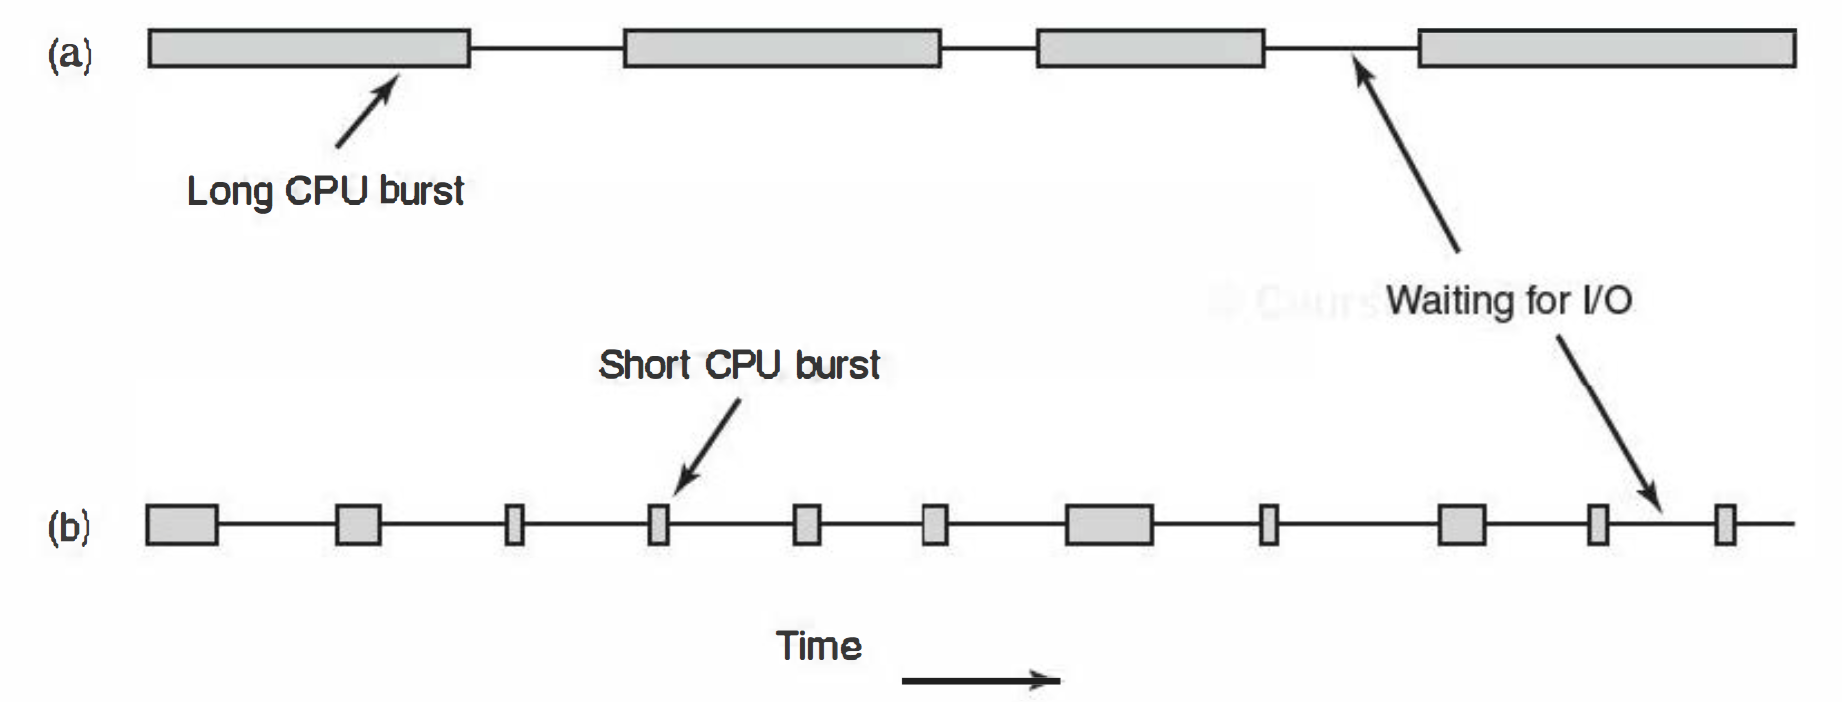
\includegraphics[width=0.75\textwidth]{images/cpu-io-bound.png}\\
CPU usage diagram showing (a) a CPU-Bound thread and (b) an I/O-Bound thread~\cite{mos}.
\end{center}

Studies have been done to examine the durations of CPU bursts. An I/O-Bound program will tend to have short CPU bursts, of course. Over time, CPUs have gotten faster at a rate much higher than the rate of I/O speedup. This is probably not surprising to you: a new CPU comes out every few months and the one you can get today is measurably better (in benchmarking tests) than the one from six months ago. I/O standards like Serial-ATA and USB and such change very slowly, over the course of years. When there \textit{is} a jump forward in I/O speed, like USB-2 to USB-3, it's often a large jump. So it makes sense that, over time, programs tend towards being I/O-Bound. The results of the study are shown below:

\begin{center}
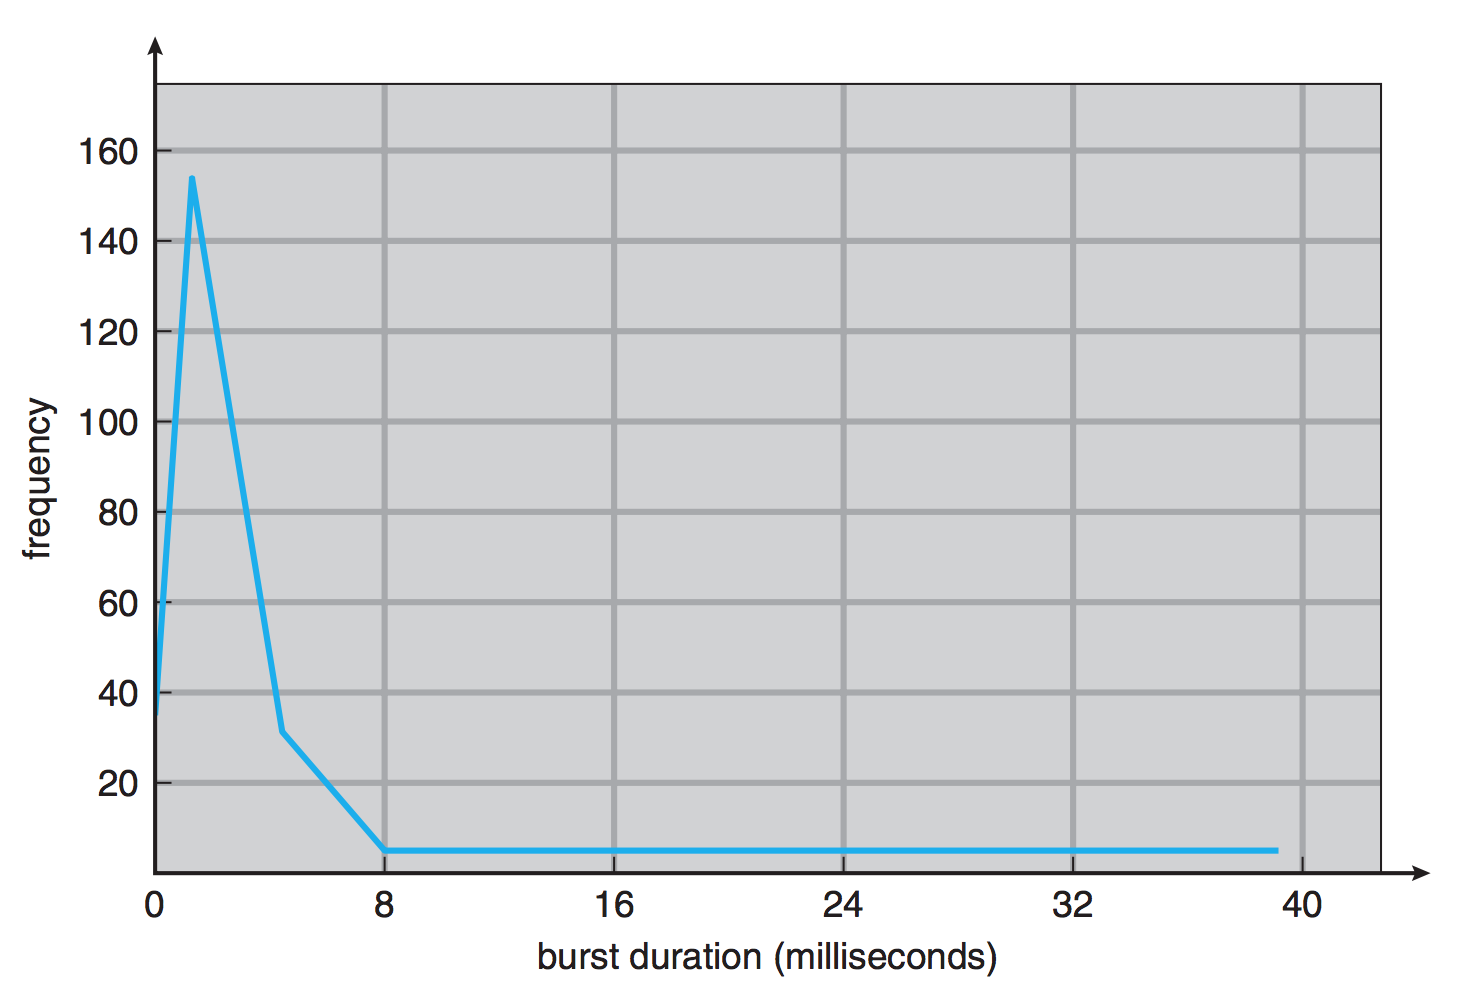
\includegraphics[width=0.65\textwidth]{images/cpu-burst-histogram.png}\\
CPU-Burst histogram~\cite{osc}.
\end{center}

But what does this have to do with scheduling? There are two ways we could make use of this. The long-term scheduler may attempt to keep a balance between CPU- and I/O-Bound tasks to get the best resource utilization. This requires that the long-term scheduler have some idea about which threads are which.

Another is that if the disk is the slowest device and the one for which we spend the most time waiting, when the disk has nothing to do, the short term scheduler should immediately schedule a thread that is likely to issue a disk request. This ensures that we do not waste any of the disk's time.

\subsection*{Scheduling Criteria}

The goals of scheduling depend significantly on the objectives of the system. If the system is supposed to respond to events within a certain period of time (real-time system), that's something you'd like to know when choosing what scheduling algorithm to implement. Perhaps the goal is for the CPU to be used maximally (as in a supercomputer). Or maybe the most important thing is for users to feel like the system answers them quickly when they issue a command.

As usual, when making a decision, we could just decide randomly, but we know that's silly here. So let's come up with some criteria to evaluate scheduling algorithms. Our goal is not to choose the one and only best algorithm, but to understand the strengths and weaknesses of each so we can choose what makes sense for our situation. We will examine the following scheduling criteria~\cite{osi}:

\begin{enumerate}
	\item Turnaround time.
	\item Response time.
	\item Deadlines.
	\item Predictability.
	\item Throughput.
	\item Processor utilization.
	\item Fairness.
	\item Enforcing priorities.
	\item Balancing resources.
\end{enumerate}

\paragraph{Turnaround Time.} The turnaround time is the amount of time between starting a thread and when it finishes. This is the execution time plus the amount of time waiting for resources (processor, I/O, etc). So, wall-clock time matters here. This is important to users; all things being equal the users would like their task to complete as fast as possible. If I ask my computer to convert a file from FLAC format to mp3 format so I can import it to my phone, I care about the turnaround time: how long will it take to convert this file?

\paragraph{Response Time.} Assuming a process is not a background process (daemon), this is the time between putting in a request and getting some answers back. A process can often start producing output while still doing the request. If I am searching for a file on disk, while the search continues to run, any results found so far can be shown in the results list. Response time is very important to users; if they click a button and it takes a long time to acknowledge the command, users get frustrated and sometimes issue the command more than once. Like the time I accidentally bought two train tickets via an Android app. Fortunately, this was a single ride ticket, so it was only a 5 Euro mistake and not a monthly ticket, which could have easily been a 100+ Euro mistake.

\paragraph{Deadlines.} This is more of a concern for real-time systems that have specific deadlines. If I am watching a movie with a Blu-Ray player, the player needs to read data from the disk, decrypt and decode it, and display it to the screen within a certain period of time, otherwise the video quality is degraded. Meeting the deadlines may be the most important thing in the system.

\paragraph{Predictability.} It is desirable if a given job runs in a fairly consistent amount of time. If a task normally takes $x$ minutes and right now it is taking $2x$ minutes, somewhere between $x$ and $2x$ minutes, the user may fear the process is stuck and might terminate it. Users are very impatient.

\paragraph{Throughput.} Scheduling policy should try to maximize the number of threads that complete in a given amount of time. This is our way of figuring out how much work is being accomplished. Much will depend here on the nature of the threads, but we would always like to get more done in the same amount of time. If I am in line to renew my drivers' license, if the Service Ontario office has a high throughput, more people will get their requests finished in the day. If it has a low throughput, I may be waiting there all day. Which would never happen. Oh no.

\paragraph{Processor Utilization.} This is, obviously, how much of the time the CPU is busy. As already mentioned, supercomputers are really expensive to build and maintain. Processing time on supercomputers is sold (leased?) to various organizations like research labs and universities. Any time the supercomputer is not in use is wasted, because that's money that we could be earning. So we may give a lot of priority to keeping it busy.

\paragraph{Fairness.} Who could be against fairness? Humans have a lot of inbuilt notions about fairness, but we are not necessarily expecting a perfectly fair routine for scheduling. What we do expect, however, is that threads should get at least a basic level of fairness, e.g., no starvation. There is a story, possibly apocryphal, about a system being shut down in 1972 that had a yet-unexecuted batch job that had been submitted some five years earlier. I think we can safely call that unfair.

\paragraph{Priorities.} Processes and threads can be assigned priorities: a way of saying that this process or thread is more or less important compared to others. Scheduling should respect this, within reasonable limits. One example of priority with reasonable limits is something like priority boarding when flying: those who get priority boarding get to get on the plane first. This has some advantages -- if overhead bin space (a resource!) is limited, getting on first helps in getting that -- but everyone who has a seat on the plane will eventually get to board and arrive at the destination.  The highest priority process/thread should probably run most often or first, but probably it should not always be the one selected, as that would violate the principle of fairness.

\paragraph{Balancing Resources.} We will get a better outcome if we balance resource usage. The example mentioned above applies: we would like to choose some CPU-Bound and I/O-Bound threads so both the CPU and I/O are kept busy. If we have more information about what sort of I/O the threads will need, so much the better: we can choose a thread that will use the printer if run, when we know the printer is idle, and avoid choosing a thread that will use the network if we know the network is busy.

\subsubsection*{Scheduling Algorithm Goals}

The priorities of these different goals depend significantly on the kind of system it is. The following list gives some idea about what is important in different kinds of systems~\cite{mos}:

\paragraph{All Systems.}
\begin{itemize}
	\item Fairness
	\item Priorities
	\item Balancing Resources
\end{itemize}

\paragraph{Batch Systems.}
\begin{itemize}
	\item Throughput
	\item Turnaround time
	\item CPU Utilization
\end{itemize}

\paragraph{Interactive Systems.}
\begin{itemize}
	\item Response time.
	\item Predictability.
\end{itemize}

\subsection*{The (Ab)use of Priorities}

Okay, so we've said that processes (and threads) have priorities and we've repeatedly referenced priority as being an important consideration in various operations like scheduling and page allocation and so on. We have not yet actually talked much about priorities.

Each process or thread's priority is typically an integer. Whether higher numbers are higher priority or lower numbers are higher priority is a question of system design. As is typical, if there are two ways to do something, some people will choose one way and some will choose the other. In UNIX, a lower number is higher priority; Windows is the opposite. Picking a convention and sticking to it would be nice, but in England they drive on the left and in Canada we drive on the right.

With a priority value assigned, it can be used to make decisions about resources. If $P_{1}$ wants resource $R_{1}$ and $P_{2}$ wants that same resource, where the priority of $P_{1}$ is greater than that of $P_{2}$, choose to assign the resource to $P_{1}$. This might come in to play, for example, when two threads are waiting on a semaphore. If process $P_{3}$ posts (signals) on the semaphore, the resource of that ``signal'' may be sent to the higher priority process $P_{1}$, allowing it to proceed first.

The operating system or the program author may each be partially responsible for assigning a priority to each of the threads. These priorities may change over time and when certain conditions are fulfilled (e.g., a process that uses a lot of CPU in a short period of time might be reassigned a lower priority by the operating system temporarily).

System administrators can usually change the priority of a thread or process. Regular users may have a say in the priority of their own threads/processes, in a limited way. In Windows, for example, as a user it may be possible to set a task to a higher or lower priority. Giving this to users was probably a bad idea, because users often do it wrong. If you have a long, CPU-Bound task, the right thing to do is to give it a low priority and not a high one. You might expect that the high priority will get the task done faster, but it hurts the performance of the system and makes users unhappy (even though that's what they explicitly asked for).

In some systems, the highest priority non-blocked thread will always run. This is a great way of making sure that higher priority threads have right-of-way, but a terrible way of ensuring fairness and preventing starvation. We could easily have a situation where low priority threads never get a chance to run, because there are too many threads of middle or high priority. So, scheduling is not necessarily as easy as just finding the highest priority thing to do...


\bibliographystyle{alphaurl}
\bibliography{350}


\end{document}